\documentclass{lab}

\title{Lab \# 2. BLE} % Title

\author{Adan Abu Naaj | adann@mit.edu \\ Artem Laptiev | laptiev@mit.edu \\\\ 6.1820} % Team # + Names, Class (RSS)

\date{\today} % Date for the report

\begin{document}

\maketitle

\newpage

\section{BLE Discovery}


\begin{figure}[h]
    \begin{center}
    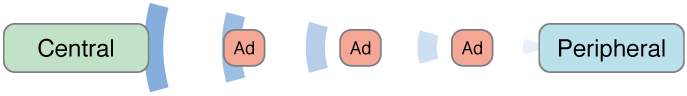
\includegraphics[width=0.65\textwidth]{images/AdvertisingAndDiscovery.png} 
    \caption{Advertising and discovery.}
    \end{center}
\end{figure}

\section{A peripheral, a service, a characteristic}

\begin{figure}[h]
    \begin{center}
    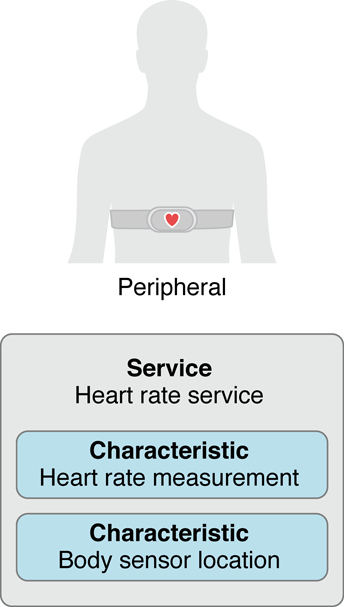
\includegraphics[height=0.25\textheight]{images/CBPeripheralData.png} 
    \caption{A peripheral’s service and characteristics.}
    \end{center}
\end{figure}

\begin{figure}[h]
    \begin{center}
    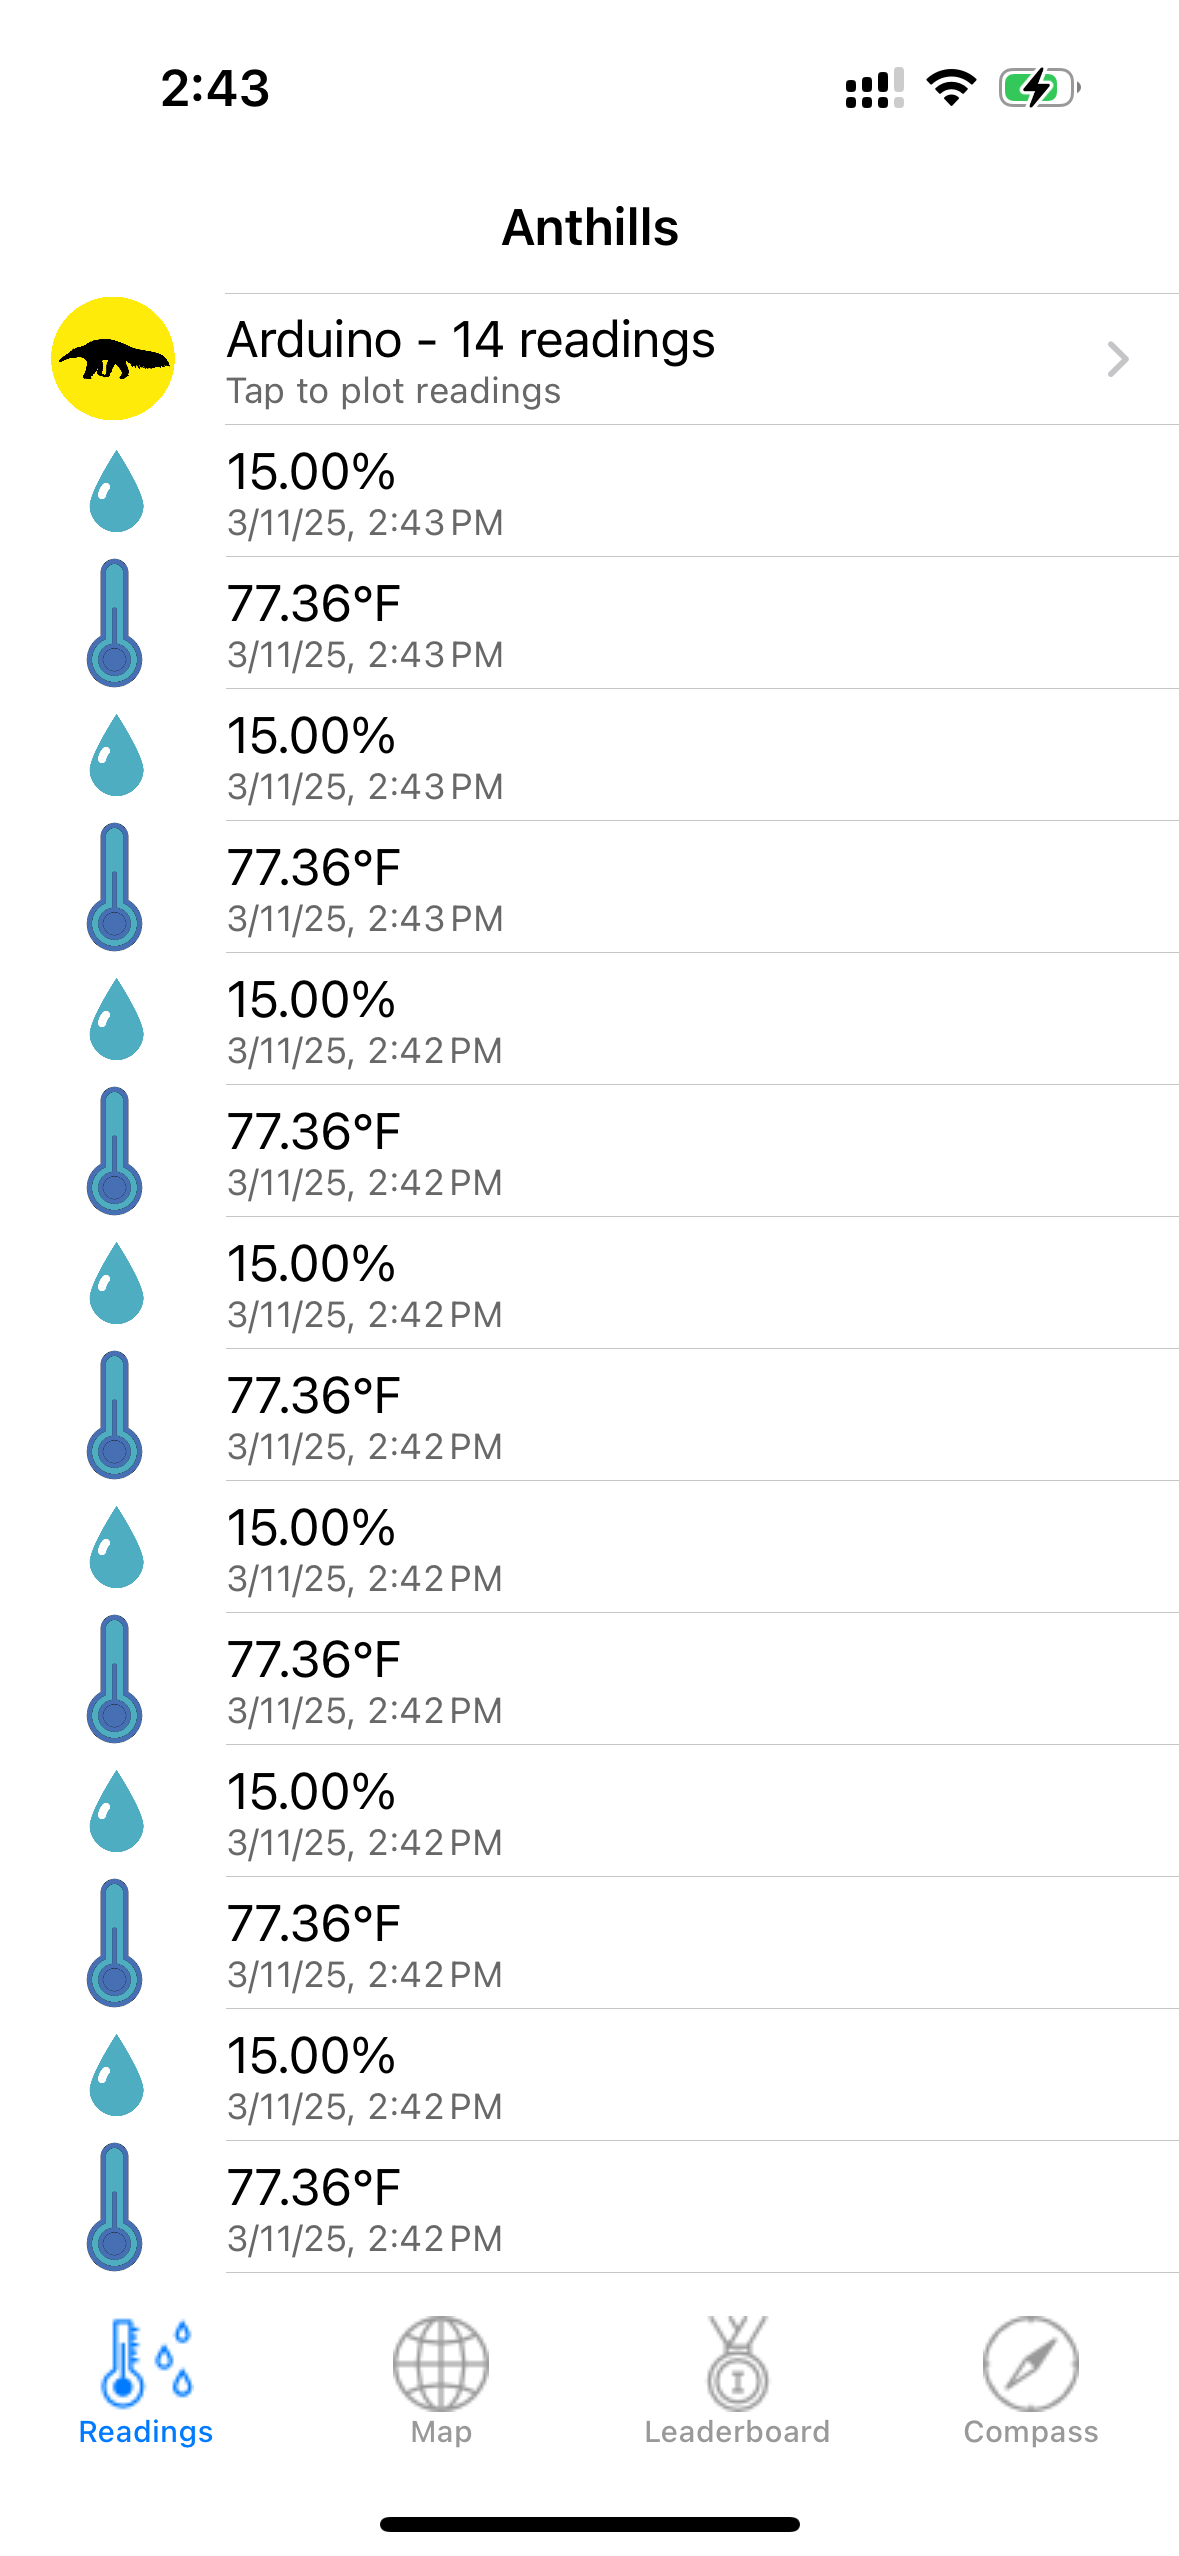
\includegraphics[height=0.35\textheight]{images/anthill.png} 
    \caption{Anthill discovered and transmitting data to client device.}
    \end{center}
\end{figure}


\section{Time Spent} 

Time spent:

% list of items:
\begin{itemize}
  \item Section 1: = 2 hour
  \item Section 2: = 1 hour
\end{itemize}


\end{document}

